\documentclass[12pt]{report}
\usepackage{amsmath, amssymb}
\usepackage{listings}
\usepackage[margin=1.6in]{geometry}
\usepackage{fancyvrb}
\usepackage{color}
\usepackage{bussproofs}
\usepackage{pgf, tikz}
\usepackage{graphicx}
\usetikzlibrary{arrows, automata}
\usepackage{hyperref}
\usepackage[scaled=.90]{helvet}
\usepackage{xcolor}
\usepackage{titlesec}

\DefineVerbatimEnvironment{blockcode}
  {Verbatim}
  {fontsize=\small,formatcom=\color{blue}}

\DefineVerbatimEnvironment{badblockcode}
  {Verbatim}
  {fontsize=\small,formatcom=\color{red}}

\titleformat{\chapter}[display]
  {\normalfont\sffamily\huge\bfseries\color{black}}
  {\thechapter.}{20pt}{\Huge}

\titleformat{\section}
  {\normalfont\sffamily\Large\bfseries\color{black}}
  {\thesection}{1em}{}

\titleformat{\subsection}
  {\normalfont\sffamily\large\bfseries\color{black}}
  {\thesubsection}{1em}{}

\fvset{%
  fontsize=\small,
  numbers=left
}

\title{\scshape Git Instruction Manual}
\author{Evan Bergeron\\
Sunny Gakhar\\
Nishad Gothoskar\\
Frederick Lee\\
Ziyang Wang
}


\begin{document}
{\sffamily \maketitle }

\tableofcontents
\newpage
\chapter{Introduction}

This is a manual on how to set up Git on your computer and set up a basic Git workflow. We cover installing, setting up, and working with git. Intermediate workflow tips are provided, as are recommendations for popular editor integrations.

This document is intended for users who want to learn Git to use it in a fast-paced setting such as a hackathon, this document is also useful as a reference for experienced Git users who want to refer to some specifc concept or command which they need.

\section{How to use this document}

Complete beginners to \texttt{git} will want to start with chapters 2 and 3. Chapter 4 covers branches; a topic perhaps not essential to basic usage. Readers already familiar with \texttt{git} may find the final chapters helpful in elevating their workflow efficiency.

\section{What is Git}

Git is a version control system designed to be used for working on small and large projects. It can be used for tracking changes between files and coordinating work on project files among multiple people.

\section{Motivation for using Git}
When you were in school and you had short homework assignments, you would just start them and finish them in a short span of time (not longer than a week). But when you move on to designing and working on bigger projects with other people, there are multiple issues that come into play. Say you are participating in a hackathon and have finalized your idea and distribution of work among the teammates. How do you actually work on the project together? 

Having all of them work on one computer is not optimal. You might have each teammate work on his own piece independently, but how do you merge everyone's work? Moreover, what if two or more teammates work on the same file, but do different modifications unknown to the others? And what if someone wants to explore a different direction to work on, while keeping the original work intact? Enter Git.

\section{Benefits of using git}
\begin{enumerate}
  \item Using Git, if you're working on a project, you can ``commit" the changes you have made and Git will keep track of all your commits. 
  
  \item If you want to explore a new direction of work which you don't want to integrate with your main project just yet, you can create a new branch and work on the branch without disturbing your main project. You can easily switch between multiple branches to work on multiple features, can when the time comes, you can merge with the main branch. 
\end{enumerate}

\chapter{Installing Git}

\section{Windows}
If you have Windows, one easy way of installing Git is from this website:

\url{https://git-scm.com/download/win}

\noindent
Once you have downloaded the installation file, you can run it and proceed through the installation steps.

\section{Mac}

Similar to Windows, one way of installing Git on is from this link

\url{https://git-scm.com/download/mac}


\noindent
Another way of installing Git is using the Xcode Command Line Tools. Open up Terminal 
and simply type \verb|git|. If you don’t have Git installed already, it will prompt you to install it.

\section{Linux}

If you're working on Linux, you can install Git using a basic package management tool that comes with your distribution.

Debian/Ubuntu

\verb|$ apt-get install git|

\bigskip

Fedora

\verb|$ yum install git| (up to Fedora 21)

\verb|$ dnf install git| (Fedora 22 and later)

\bigskip

Arch Linux

\verb|$ pacman -S git|

\bigskip

FreeBSD

\verb|$ pkg install git|

\bigskip

Solaris 9/10/11 (OpenCSW)

\verb|$ pkgutil -i git|

\bigskip

Solaris 11 Express

\verb|$ pkg install developer/versioning/git|

\bigskip

OpenBSD

\verb|$ pkg_add git|


\chapter{Getting Started}
\section{Initializing Repository}

To make sure you have Git set up, type \verb|git| into your console (Terminal for Mac/Linux users and Command Prompt for Windows users) and the following should show up (the full output has been elided here).

\begin{blockcode}
$ git
usage: git [--version] [--help] [-C <path>] [-c name=value]
[--exec-path[=<path>]] [--html-path] [--man-path] [--info-path]
[-p | --paginate | --no-pager] [--no-replace-objects] [--bare]
[--git-dir=<path>] [--work-tree=<path>] [--namespace=<name>]
<command> [<args>]

...

'git help -a' and 'git help -g' list available subcommands and some
concept guides. See 'git help <command>' or 'git help <concept>'
to read about a specific subcommand or concept.
\end{blockcode}
\bigskip
\noindent
To start a new repository, first go to ttype \verb|git init| into the console. It should output the following:

\begin{blockcode}
$ git init
Initialized empty Git repository in <path to current directory>/.git/
\end{blockcode}

\bigskip
\noindent
This creates a \verb|./git| directory in your current directory, which consists of all information about the repository. It consists of a HEAD file, which points to the current version of the repository.


\section{Adding files to version control}

The staging environment, or sometimes referred as index, is a file that stores information that you want to edit to the git repository. After you have initialized a repository, you may want to add new files to the repository. However, git does not know which files you want to include in the staging environment. \texttt{git add} command is used for adding files to the staging environment.

For example, after creating a \texttt{test.txt} file in your working directory, you can check the current status using \texttt{git status} command. You should get the following message:

\begin{blockcode}
$ git status
On branch master
Untracked files:
  (use "git add <file>..." to include in what will be committed)
  
    test.txt

nothing added to commit but untracked files present
(use "git add" to track)
\end{blockcode}

In order to add the file to the staging environment and notify git for this change, type \texttt{git add test.txt} and check status. You should get the following message:

\begin{blockcode}
$ git add test.txt
$ git status
On branch master
Changes to be committed:
  (use "git reset HEAD <file>..." to unstage)
  
    New file: test.txt

\end{blockcode}

Now the new file is ready for commit, i.e. ready to be added to the git repository.

If the file you want to add is not in the working directory, use \texttt{git add <pathspec>} instead to add the file to the staging environment.

\section{Committing changes}

A commit is a record of what files you have added or changed since the last time you committed changes. Running the command \texttt{git commit -m "Message for the commit"} creates a new commit for all the changes you have made. The message after you creating the commit should contain relevant information about the changed you made.

For example, if you changed some contents in the file \texttt{index.html} and created a new file \texttt{new.txt}, a commit message should look like something as following:

\begin{blockcode}
$ git commit -m "Change index, add new file"
[master 3651e36] Change index, add new file
2 files changed, 10 insertions(+)
create mode 100644 new.txt
\end{blockcode}

The \texttt{"-m"} flag allows you to give a message without opening a text editor. Alternatively, using \texttt{git commit} will open your text editor with some message like the following:

\begin{blockcode}
$ git commit
# Please enter the commit message for your changes. Lines starting
# with '#' will be ignored, and an empty message aborts the commit.
# On branch master
# Your branch is up-to-date with 'origin/master'.
#
# Changes to be committed:
# new file:   new.txt
# modified:   index.html
#
~
~
~
".git/COMMIT_EDITMSG" 9L, 283C
\end{blockcode}


It is worth noting that anything that is still unstaged (files you have created or modified that you haven’t run git add on since you edited them) won’t go into the commit. 

Creating a commit does not change any remote repository. If you are using GitHub, you probably want this commit changes respective contents in the remote repository on GitHub. You can use \texttt{git push} to update remote repository with committed changes.

\begin{blockcode}
$ git push
\end{blockcode}

\section{Reverting changes}

One reason people using git as version control is that it can undo changes easily. When you make a new commit, git stores the status of your repository at that specific moment. In the future, you can go back to an earlier version by going back to the status git stored.

Here are several undo commands and the scenarios for using them:

\begin{enumerate}
  \item \texttt{git revert <SHA>}. You have used \texttt{git push} to change your remote repository, but want to undo the change. This command creates a new commit that does the inverse of the given SHA. In other words, it undoes the previous commit by giving opposite changes.
  \item \texttt{git commit --amend}. You created a new commit but have not pushed it to remote repository. There is a typo in your commit message. This command allows you to retype the commit message.
  \item \texttt{git checkout -- <filename>} You want your files to go back to the state in the last commit. \texttt{git checkout} changes file in the working directory to a state previously recorded by git.
  \item \texttt{git reset <SHA>}. You created several commits but have not pushed them to remote repository. The changes you made in the last commit is horrible and you want to go back to certain commit. \texttt{git reset} rewinds your repository's history back to the specified \texttt{<SHA>}.
  \item \texttt{git reflog}. You used \texttt{git reset} to undo changes, but now you want redo them. \texttt{git reflog} recovers your directory's history.
\end{enumerate}
\section{Ignoring Files}

The best way to ignore files in a repository is to create a \texttt{.gitignore} file at the base of your repository with the names of all files to ignore.

Often you will find that in your projects, you will have files in your repository that do not need to be tracked.  These include automatically generated files, larger libraries that are really external dependencies, or system specific files such as the \texttt{.DS\_Store} file in Macs.

For example, let us have a repository with two files: \texttt{code.py} and \texttt{generated.txt}.  Here we only want to keep track of changes to \texttt{code.py} while ignoring changes to \texttt{generated.txt} which is automatically generated every time \texttt{code.py} is run.

Without a \texttt{.gitignore} file, running \texttt{git status} would get the following output:

\begin{blockcode}
$ git status
On branch master
Untracked files:
  (use "git add <file>..." to include in what will be committed)
  
    code.py
    generated.txt

nothing added to commit but untracked files present
(use "git add" to track)
\end{blockcode}

We create a \texttt{.gitignore} file with the following content:

\begin{blockcode}
generated.txt
.gitignore
\end{blockcode}

Running \texttt{git status} again, we see that the generated file and the \texttt{.gitignore} itself are ignored by Git as desired.

\begin{blockcode}
$ git status
On branch master
Untracked files:
  (use "git add <file>..." to include in what will be committed)
  
    code.py

nothing added to commit but untracked files present
(use "git add" to track)
\end{blockcode}

\chapter{Branching}

In git, branching is used to keep track of the different paths of development for your project.  The master branch is the main branch of your project and after features or changes are verified, they are usually added to the master branch of the project.

\section{Creating branches}

To create a new branch (for example if you want a new branch named addfeature):
\begin{blockcode}
$ git branch add_feature
\end{blockcode}
  
This creates a new branch in the “development tree”.  Now you can work on this branch of the project without effecting the master branch.


As the figure above shows, branching creates a separate flow.  Now in order to bring your current local state to that branch you will have to check it out by:

\begin{blockcode}
$ git checkout add_feature
\end{blockcode}  

Now the changes you make will be modifying this new branch rather than the master branch.  To go back to the master branch you will use the same checkout command with master rather than addfeature.

Note that to checkout a different branch your current changes must be committed or stored away before you can switch.

A simple shortcut is to run:

\begin{blockcode}
$ git checkout -b add_feature
\end{blockcode}  

Note that to checkout a different branch your current changes must be committed or stored away before you can switch.

Now when you are done with development you can delete your branch by using:

\begin{blockcode}
$ git branch -d add_feature
\end{blockcode}  

If you want to rollback and see the state of your project at some previous point, you can use git log to look at the commit history and find the commit hash 

 

and use:

\begin{blockcode}
$ git checkout 1c0191a6a6264f2e90f6905636321fde897b86df
\end{blockcode}  

To checkout the previous commit and see the state of the project at that point.

To combine branches, we have two main options: merging and rebasing.

\section{Merging Branches}

Now after working on these separate branch and adding your new feature, you want to merge this work into your master branch so it will persist and new branches can build upon or use the feature you added.  This is what merging does.  It takes a branch and “merges” it into another branch.  This can be done by first checking out the branch you want to merge INTO:

\begin{blockcode}
$ git checkout master
\end{blockcode}  

And then merging the other branch in by:

\begin{blockcode}
$ git merge add_feature
\end{blockcode}  
This may happen immediately, unless there are conflicts between the two branches that need to be resolved before they can be successfully merged.  By using git status, you can see in which files these conflicts are located.  Then within the files you will find sections of the form:

\begin{blockcode}
<<<<< HEAD
stuff in the current branch
=====
things in other branch
>>>>> add_feature
\end{blockcode}  

And you will have to replace these sections with the content you want and then commit the changes to fully process the merge of the two branches.

\section{Rebasing Branches}

The rebasing and merging are the two primary ways of combining changes from separate branches with Git.  One primary advantage of rebasing is that the Git history is made more linear which makes it easier to track changes over time.

For example, say that you have been working on a separate branch called \texttt{feature} (shown in blue) on which you have two commits.  At the same time, a friend of yours has committed change ``C" to master (shown in green).

\begin{figure}[h]
\center
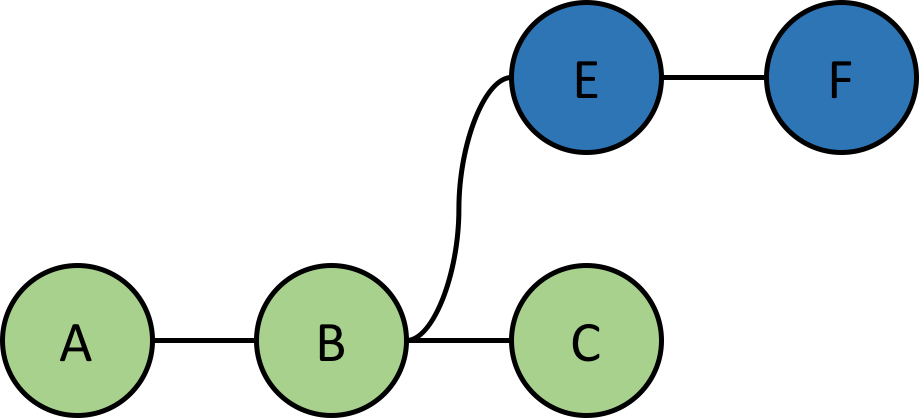
\includegraphics[height=2cm]{feature}
\end{figure}

A regular merge command such as
\begin{blockcode}
$ git checkout master
$ git merge feature
\end{blockcode}
would result in the following Git history:
\begin{figure}[h]
\center
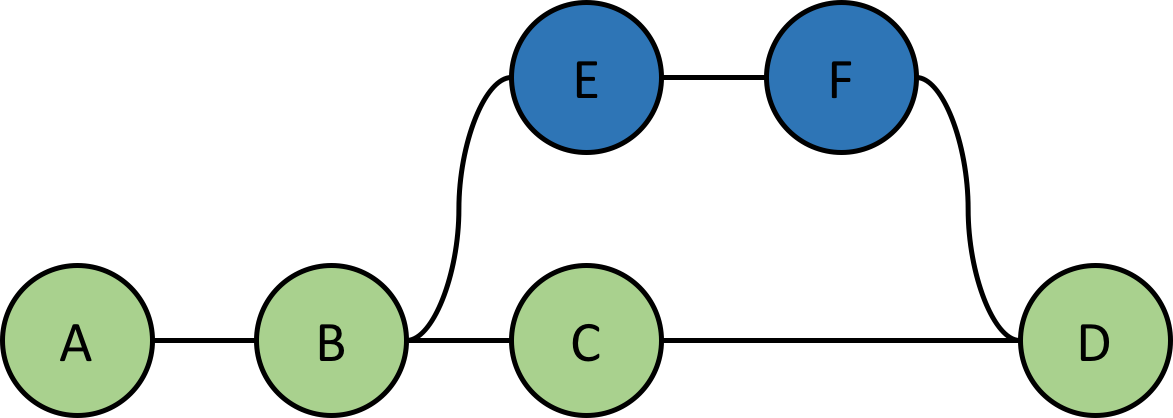
\includegraphics[height=2cm]{merge}
\end{figure}

However, if you want a more linear history, you would ideally want your commits ``E" and ``F" to be stacked on top of your friends commits.  To do as such, simply run as follows:
\begin{blockcode}
$ git checkout feature
$ git rebase master
$ git checkout master
$ git merge feature
\end{blockcode}

The initial rebase command changes the root of your \texttt{feature} branch to your friend's last commit as shown below on the left image.

\begin{figure}[h]
\center
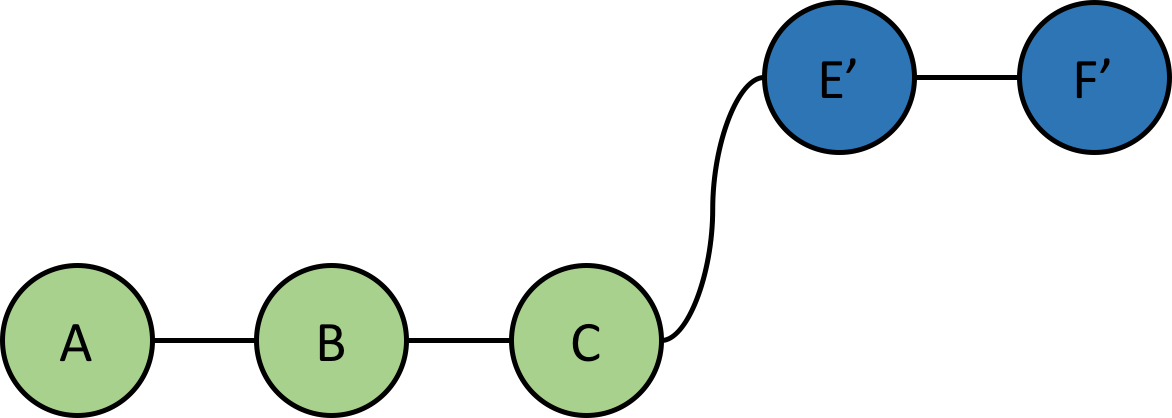
\includegraphics[height=2cm]{rebase}
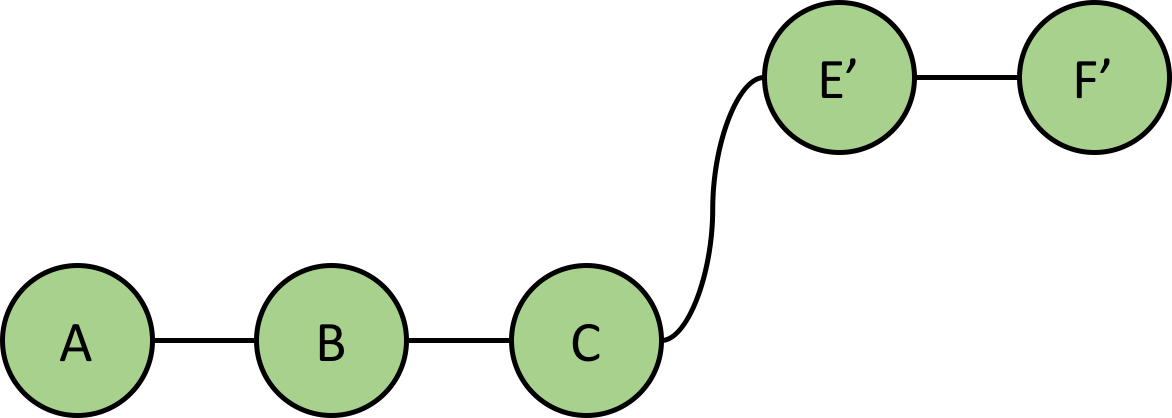
\includegraphics[height=2cm]{rebase_merge}
\end{figure}

The final merge of your feature onto master then forwards master's history to match your feature branch as shown above on the right.  As you can see, the history follows a much more linear pattern compared to the branching pattern of a regular merge alone.

\chapter{Intermediate Git}
\section{Cherry-picking Commits}

Cherry-picking is particularly useful when you don't want to apply all changes from a branch to another branch through a merge or rebase, but only want to apply a few specific commits.

For example, take the hypothetical situation where your most recent commit ``F" in your feature branch (shown in blue) is suffering from a application-breaking bug, but your manager wants your changes in commit ``E" to be rolled out by this afternoon.

\begin{figure}[h]
\center
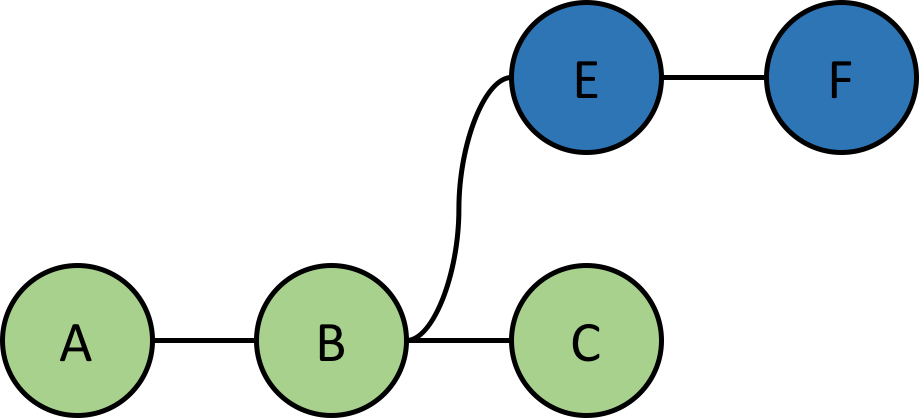
\includegraphics[height=2cm]{feature}
\end{figure}

To apply commit ``E" by itself to the master branch (in green), first find the commit-hash of your desired commit by running \texttt{git log} and searching for your commit.  A commit-hash is an identifying string of letters and numbers that may look something like \texttt{f3def414605008d5c899b2691ff1b6d1d3798a0a}.  After you have found your commit-hash, to apply your desired commit to the master branch, run the following commands:
\begin{blockcode}
$ git checkout master
$ git cherry-pick <commit-hash of E>
\end{blockcode}

Running these commands gets your final desired result shown below:

\begin{figure}[h]
\center
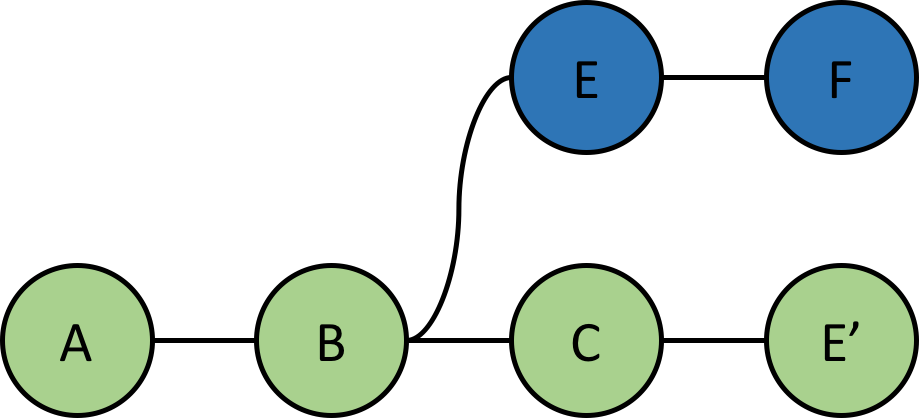
\includegraphics[height=2cm]{cherrypick}
\end{figure}

where commit ``E" has been applied to the master branch from your feature branch without merging your entire bug-ridden feature branch to master.

\section{Collaboration with Github}

You can use github for a more user-friendly version controlling experience.  Almost everything you can do using the command line can be done using the desktop client.  You can easily select files, read their diffs, and commit them.
 

Using the online interface, you can create repositories, add contributors, and track progress very easily.

The workflow using github usually involves many collaborators who make pull requests to the managers of the repository.


\section{Easily Reordering Commits}

Reordering commits is a common task and can be performed in a single command. 
A naive workflow for this task might look like
\begin{badblockcode}
$ git checkout -b tmp
$ git checkout master
$ git reset --hard HEAD~
$ git cherry-pick tmp
\end{badblockcode}

This works fine, but there’s a simpler method. We can simply say:
\begin{blockcode}
$ git rebase -i HEAD~2
\end{blockcode}
This will open an interactive git rebasing session (the \texttt{-i}
stands for interactive). The window will display something along the
lines of
\begin{blockcode}
pick 370e221 Commit one
pick c342396 Commit two
\end{blockcode}
Simply reorder these lines to reorder the commits. Much shorter!

\section{Adding partial files}
It can sometimes be helpful to stage only part of the changes made to a single file. (Especially if there are two logically different salient tasks). A naive workflow might involve creating separate branches and manually editing files. Instead, we may say:

\begin{blockcode}
$ git add -p <file>
\end{blockcode}
This will bring up an interactive prompt. This prompt will cycle
through the different areas of the diff. For each section, you will be asked if you want to stage each section. You may hit \texttt{y} or \texttt{n} for yes or no.

Once you're done adding the subset of changes you want to commit, you
can double-check you have the right changes staged by saying
\begin{blockcode}
$ git diff --cached
\end{blockcode}
One everything looks good, simply \texttt{commit} as normal.

\section{Git aliases}
Typing out full commands such as ``\texttt{git commit}'' and ``\texttt{git log --oneline}'' can take a lot of time. Git aliases are a useful tool to save yourself commonly typed commands. For instance, we might say
\begin{blockcode}
$ git config --global alias.l "log --oneline"
$ git l
\end{blockcode}
to save ourselves typing out ``\texttt{log --oneline}'' everytime. It is worth spending a couple moments to create a handful of shortcuts.

\chapter{Vim Integration}

At the time of writing, perhaps the most feature complete vim-git
plugin is Tim Pope’s “vim-fugitive.” Consequently, we will assume
usage of this plugin throughout the entire vim workflows tutorial.

\section{Installing vim-fugitive}

There are a number of ways to install vim-fugitive. The one suggested
by Tim Pope is as follows:
\begin{blockcode}
$ cd ~/.vim/bundle
$ git clone git://github.com/tpope/vim-fugitive.git
$ vim -u NONE -c "helptags vim-fugitive/doc" -c q
\end{blockcode}
Vundle is a great plugin manager for vim -- if you use this, you may
simply add the line
\[
  \texttt{Plugin 'tpope/vim-fugitive}
\]
to your vimrc and run the \texttt{PluginInstall} command.

\section{Easy git blame}
You’re browsing some file and discover a horrible bug written by one
of your coworkers. You’re about to storm over to someone’s desk and
verbally abuse them for producing incorrect code. Before you deliver
your diatribe, you need to know who to blame.

Before using \texttt{vim-fugitive}, you would have to exit vim,
manually type “\texttt{git blame <filename>},” and then search for the
relevant line in the output. Now, you can simply type
“\texttt{:Gblame}” in your vim prompt, and a vertical split will open
up right next to the line in question. You could even establish a
keybinding to do this for you! What was once several lines of typing
is now a single keystroke away! Your coworkers have never been so
scared\ldots

% TODO Evan will finish this in a later draft
\chapter{Emacs Integration}

Similarly to vim-fugitive for vim, “Magit” is (at the time of
writing), the most feature-complete git wrapper for emacs. We will
thus assume usage of this package.

\section{Installing Magit}
Perhaps the easiest way to install is through MELPA. Just run
\[
  \texttt{M-x package-install RET magit RET}
\]

\section{Using Magit}
We only have space to cover the basics of git usage in magit, but
here’s a general outline:

\end{document}
